Rysunki ~\ref{fig:rys1} - ~\ref{fig:rys5} przedstawiają wykresy dla lasera VCSEL 850\,nm. \\
\begin{table}
\begin{center}
\caption{ Wyznaczone wartośc prądu progowego $I_{\mathrm{th}}$ w różnych temperaturach $T$ dla lasera VCSEL 850\,nm. }
\begin{tabular}{ | C{1.5cm}|  C{3.0cm} | C{1.5cm} | C{3.0cm}| C{1.5cm} | C{3.0cm}|}
\hline
$T$ [K] &   $I_{\mathrm{th}}$ [mA]  &  $T$ [K] &   $I_{\mathrm{th}}$ [mA]  &  $T$ [K] &   $I_{\mathrm{th}}$ [mA] 	\\ \hline
283      &   1.70 $\pm$ 0.03  & 288      &   1.67 $\pm$ 0.03   & 293		 &   1.60 $\pm$ 0.03  \\ \hline
298		 &   1.55 $\pm$ 0.04  & 303		 &   1.59 $\pm$ 0.03  & 308		 &   1.63 $\pm$ 0.03  \\ \hline
313		 &   1.65 $\pm$ 0.03  & 318		 &   1.68 $\pm$ 0.04  & 323		 &   1.73 $\pm$ 0.04  \\ \hline
328		 &   1.83 $\pm$ 0.04  & 333		 &   1.89 $\pm$ 0.04  & 338		 &   2.01 $\pm$ 0.04  \\ \hline
343		 &   2.14 $\pm$ 0.04  & 348		 &   2.24 $\pm$ 0.05  & 353		 &   2.38 $\pm$ 0.05  \\ \hline
358		 &   2.57 $\pm$ 0.05  & 363		 &   2.74 $\pm$ 0.07  \\ \cline{1-4}
\end{tabular}
\end{center}
\end{table}
\begin{figure}
\center
  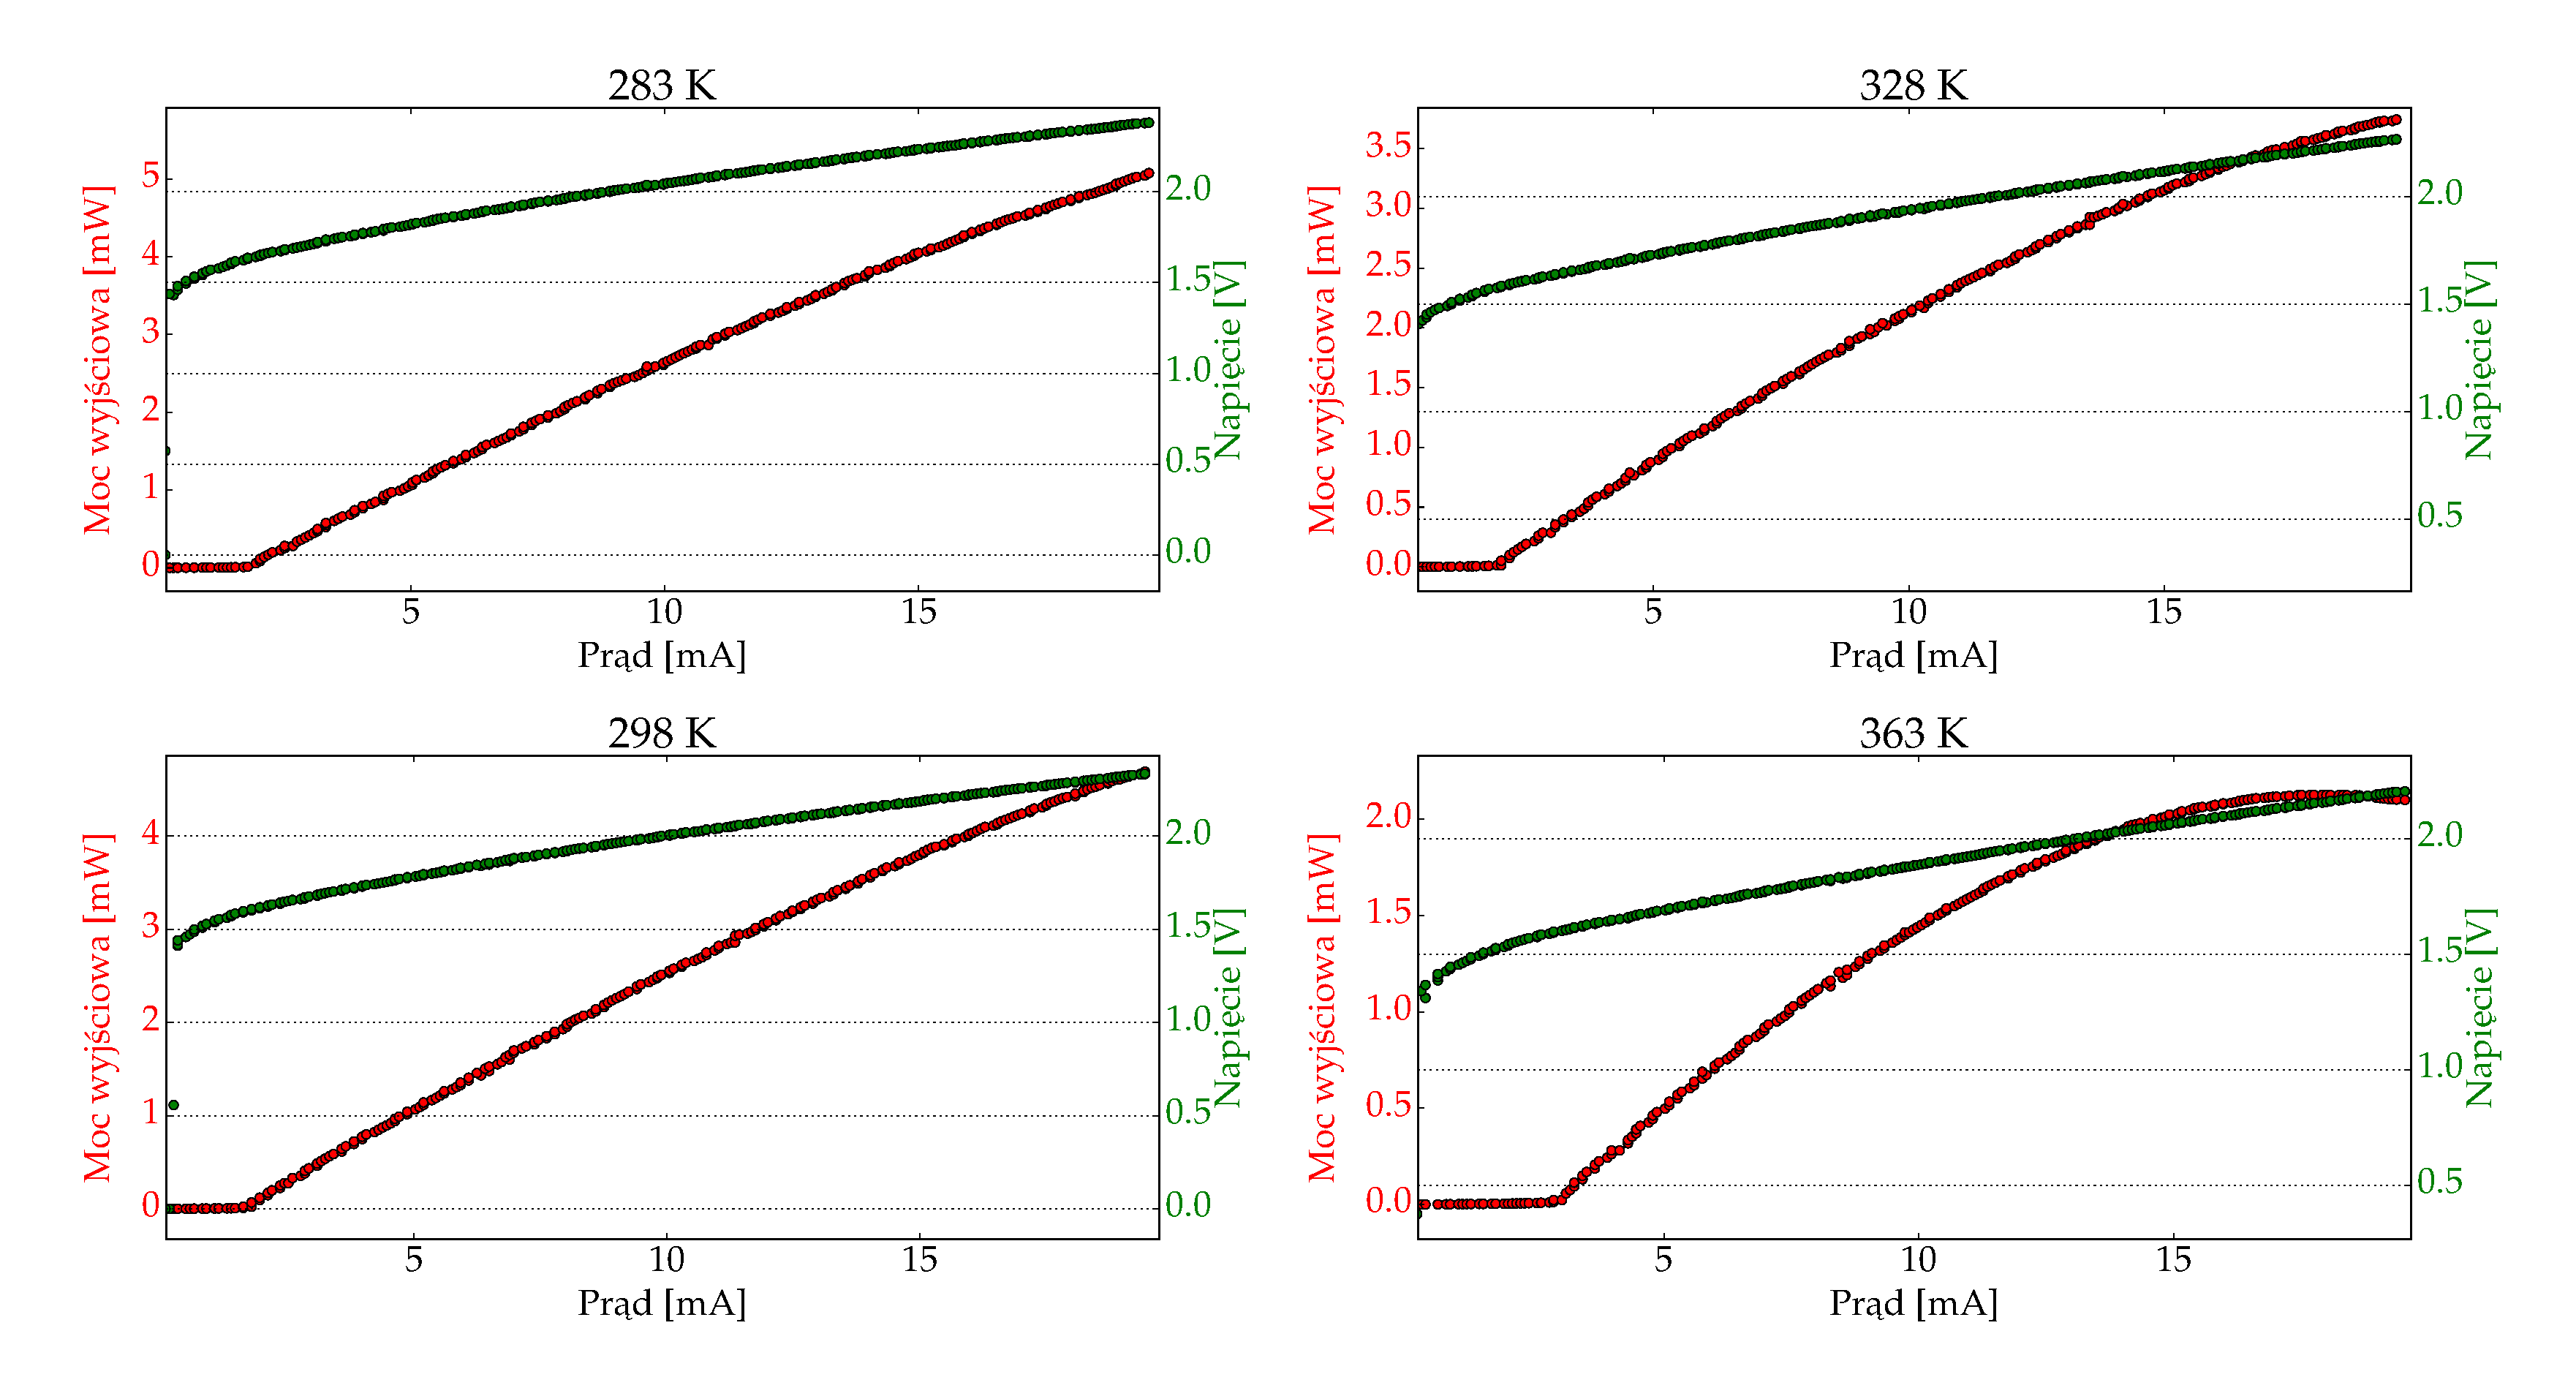
\includegraphics[scale=0.30]{plot_vcsel_850/plot_ivl_4.eps}
  \caption{Sprawność VCSEL 850.} 
  \label{fig:rys1}
\end{figure}
\begin{figure}
\center
  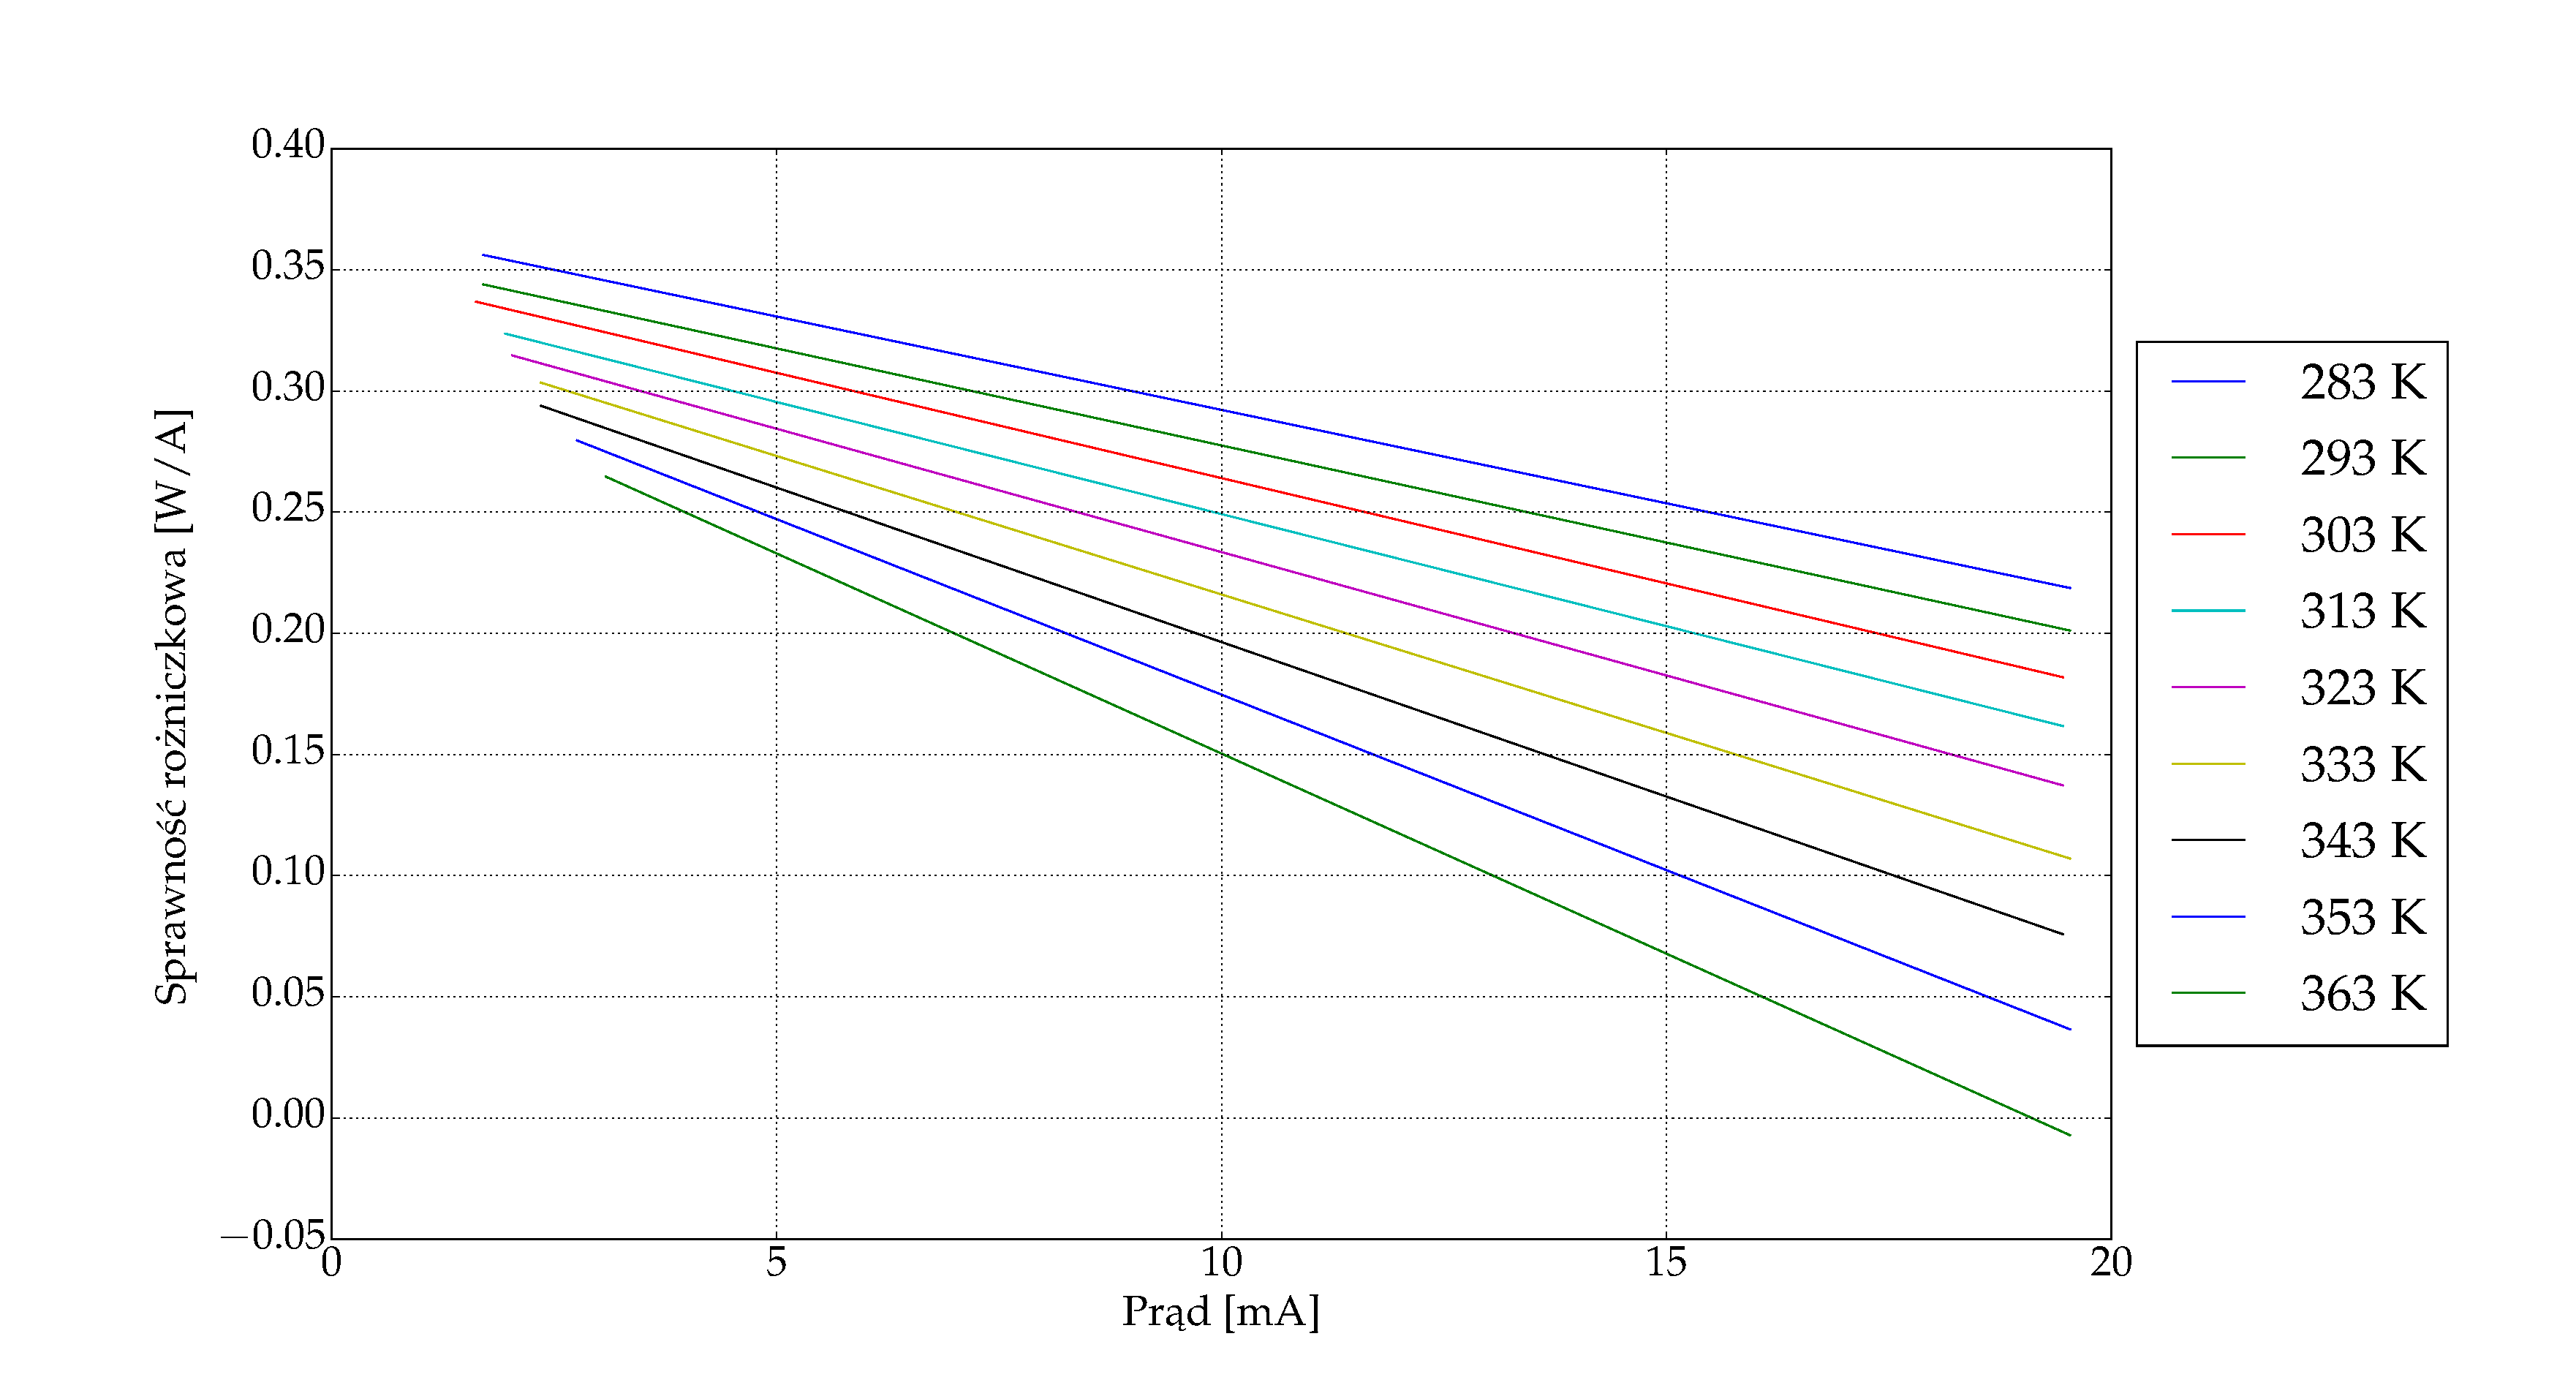
\includegraphics[scale=0.30]{plot_vcsel_850/plot_eff_all_via_current.eps}
  \caption{Sprawność VCSEL 850 w funkcji prądu.}
  \label{fig:rys2}
\end{figure}
\begin{figure}
\center
  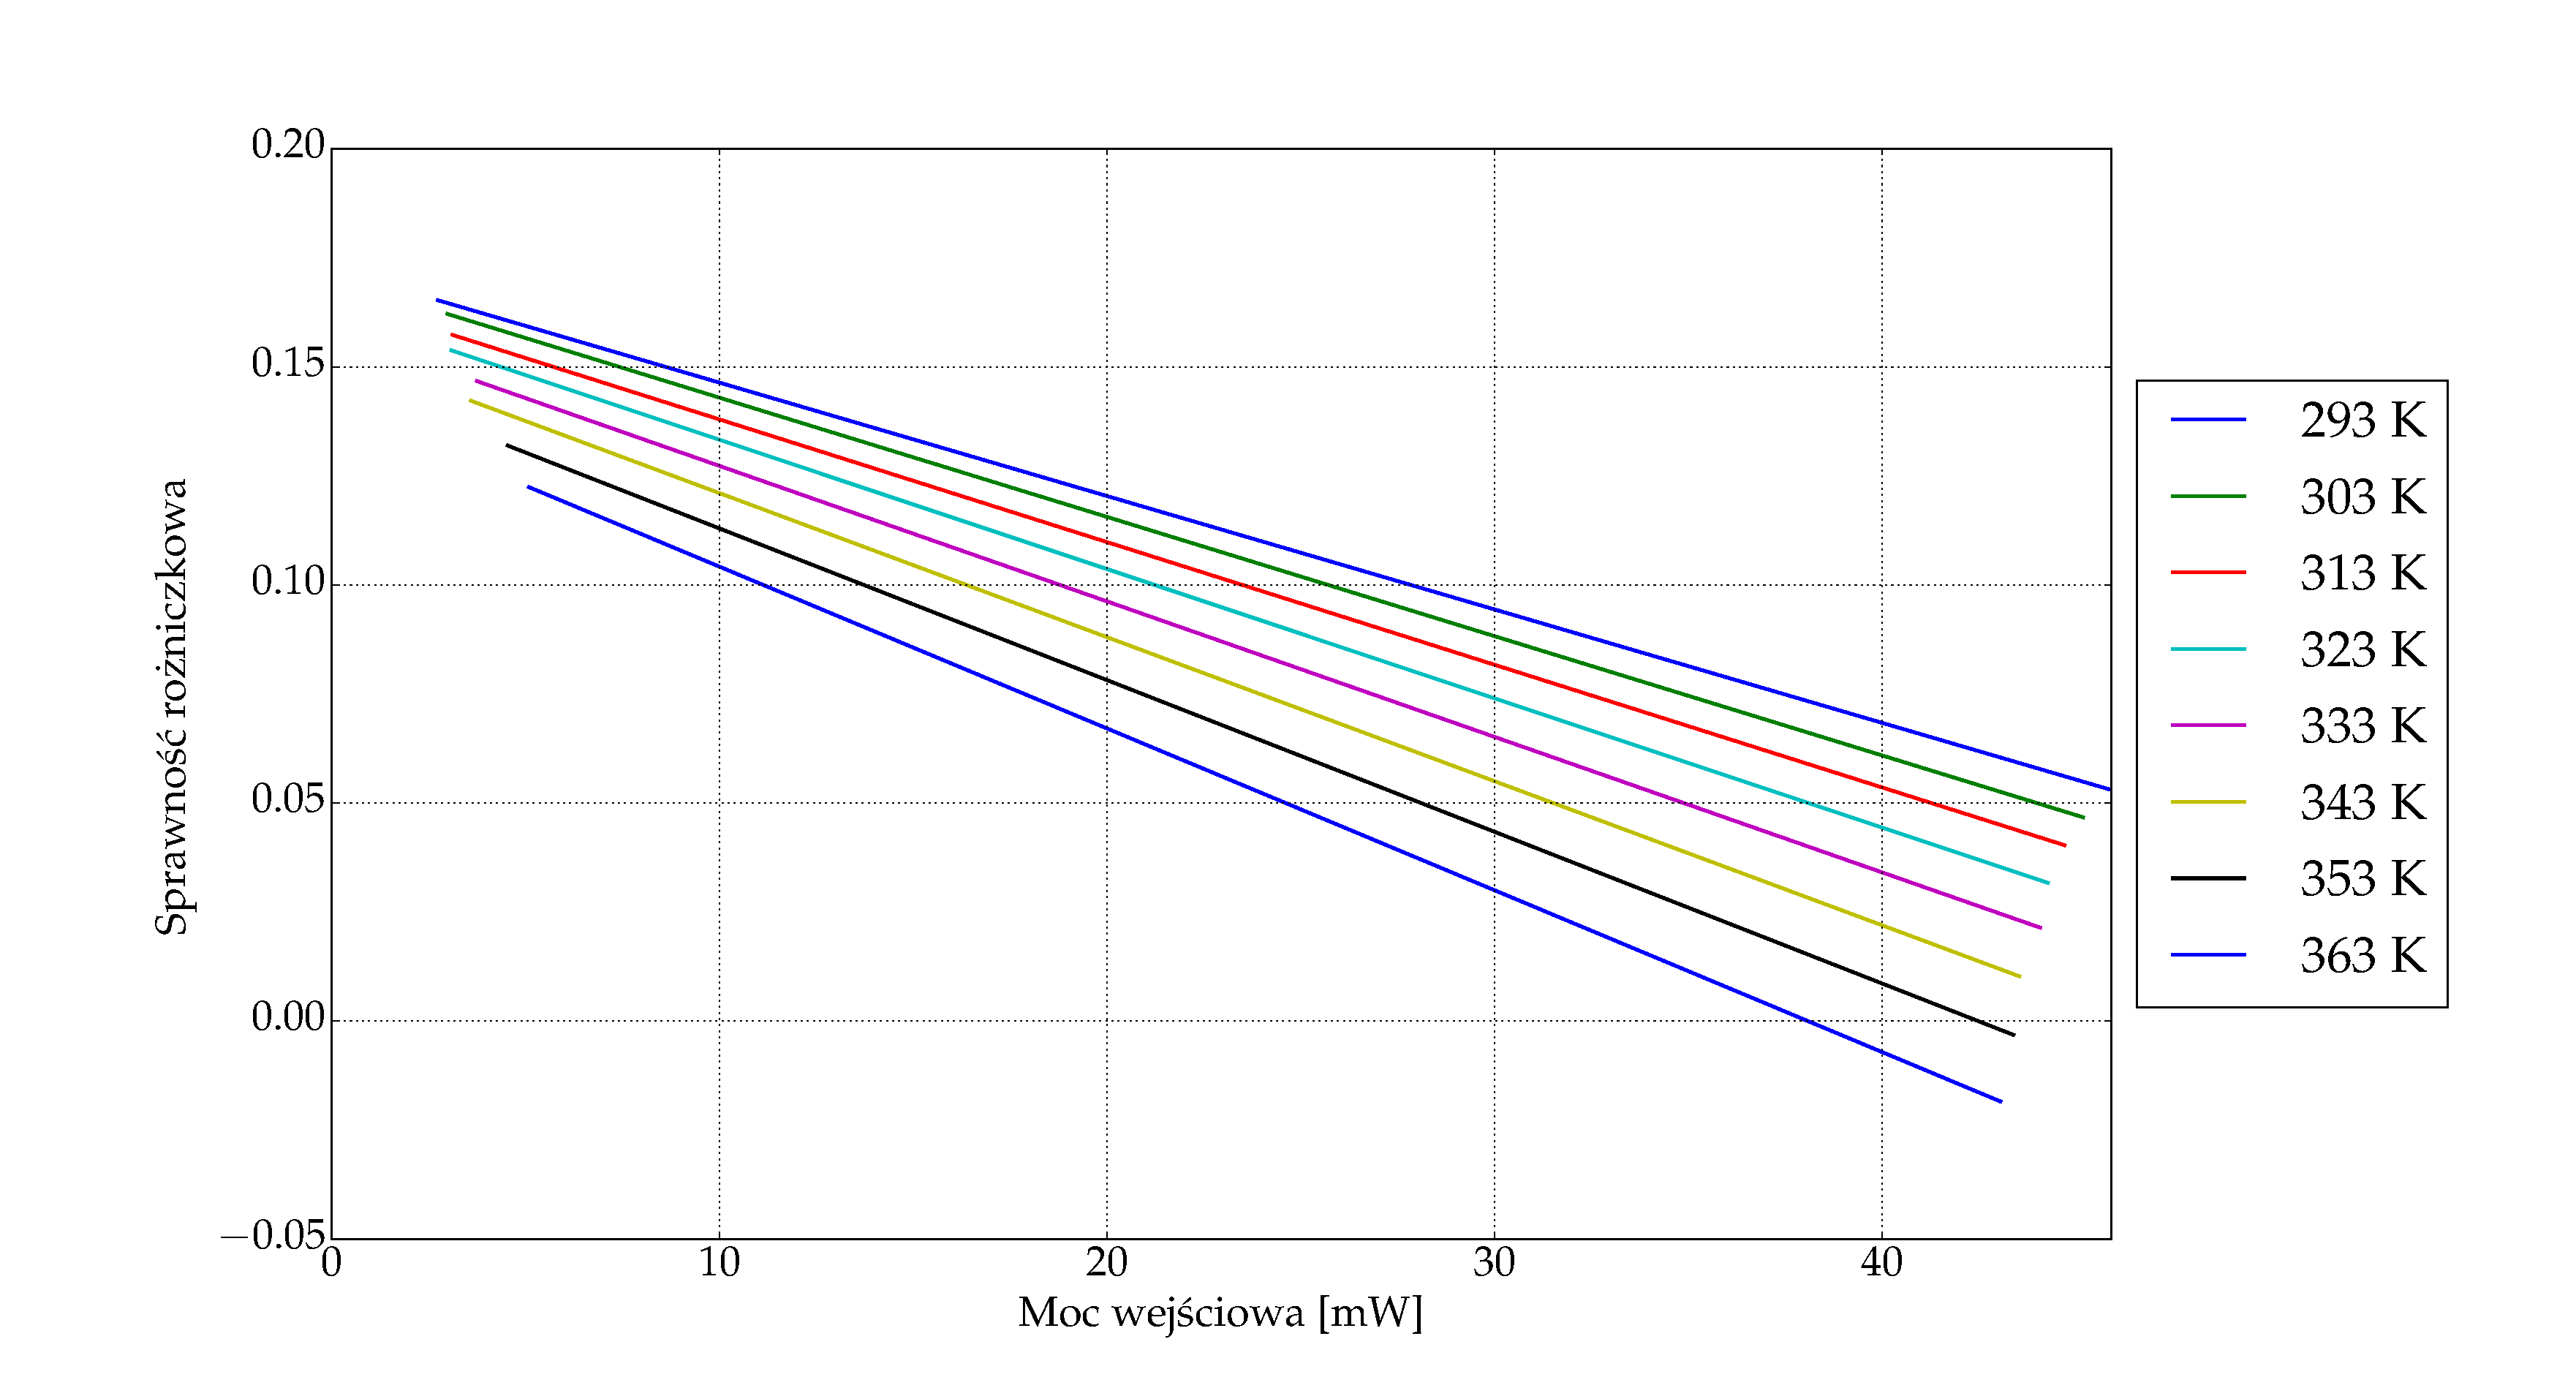
\includegraphics[scale=0.30]{plot_vcsel_850/plot_eff_all_via_power.eps}
  \label{fig:rys3}
  \caption{Sprawność VCSEL 850 w funkcji mocy wejściowej.}
\end{figure}
\begin{figure}
\center
  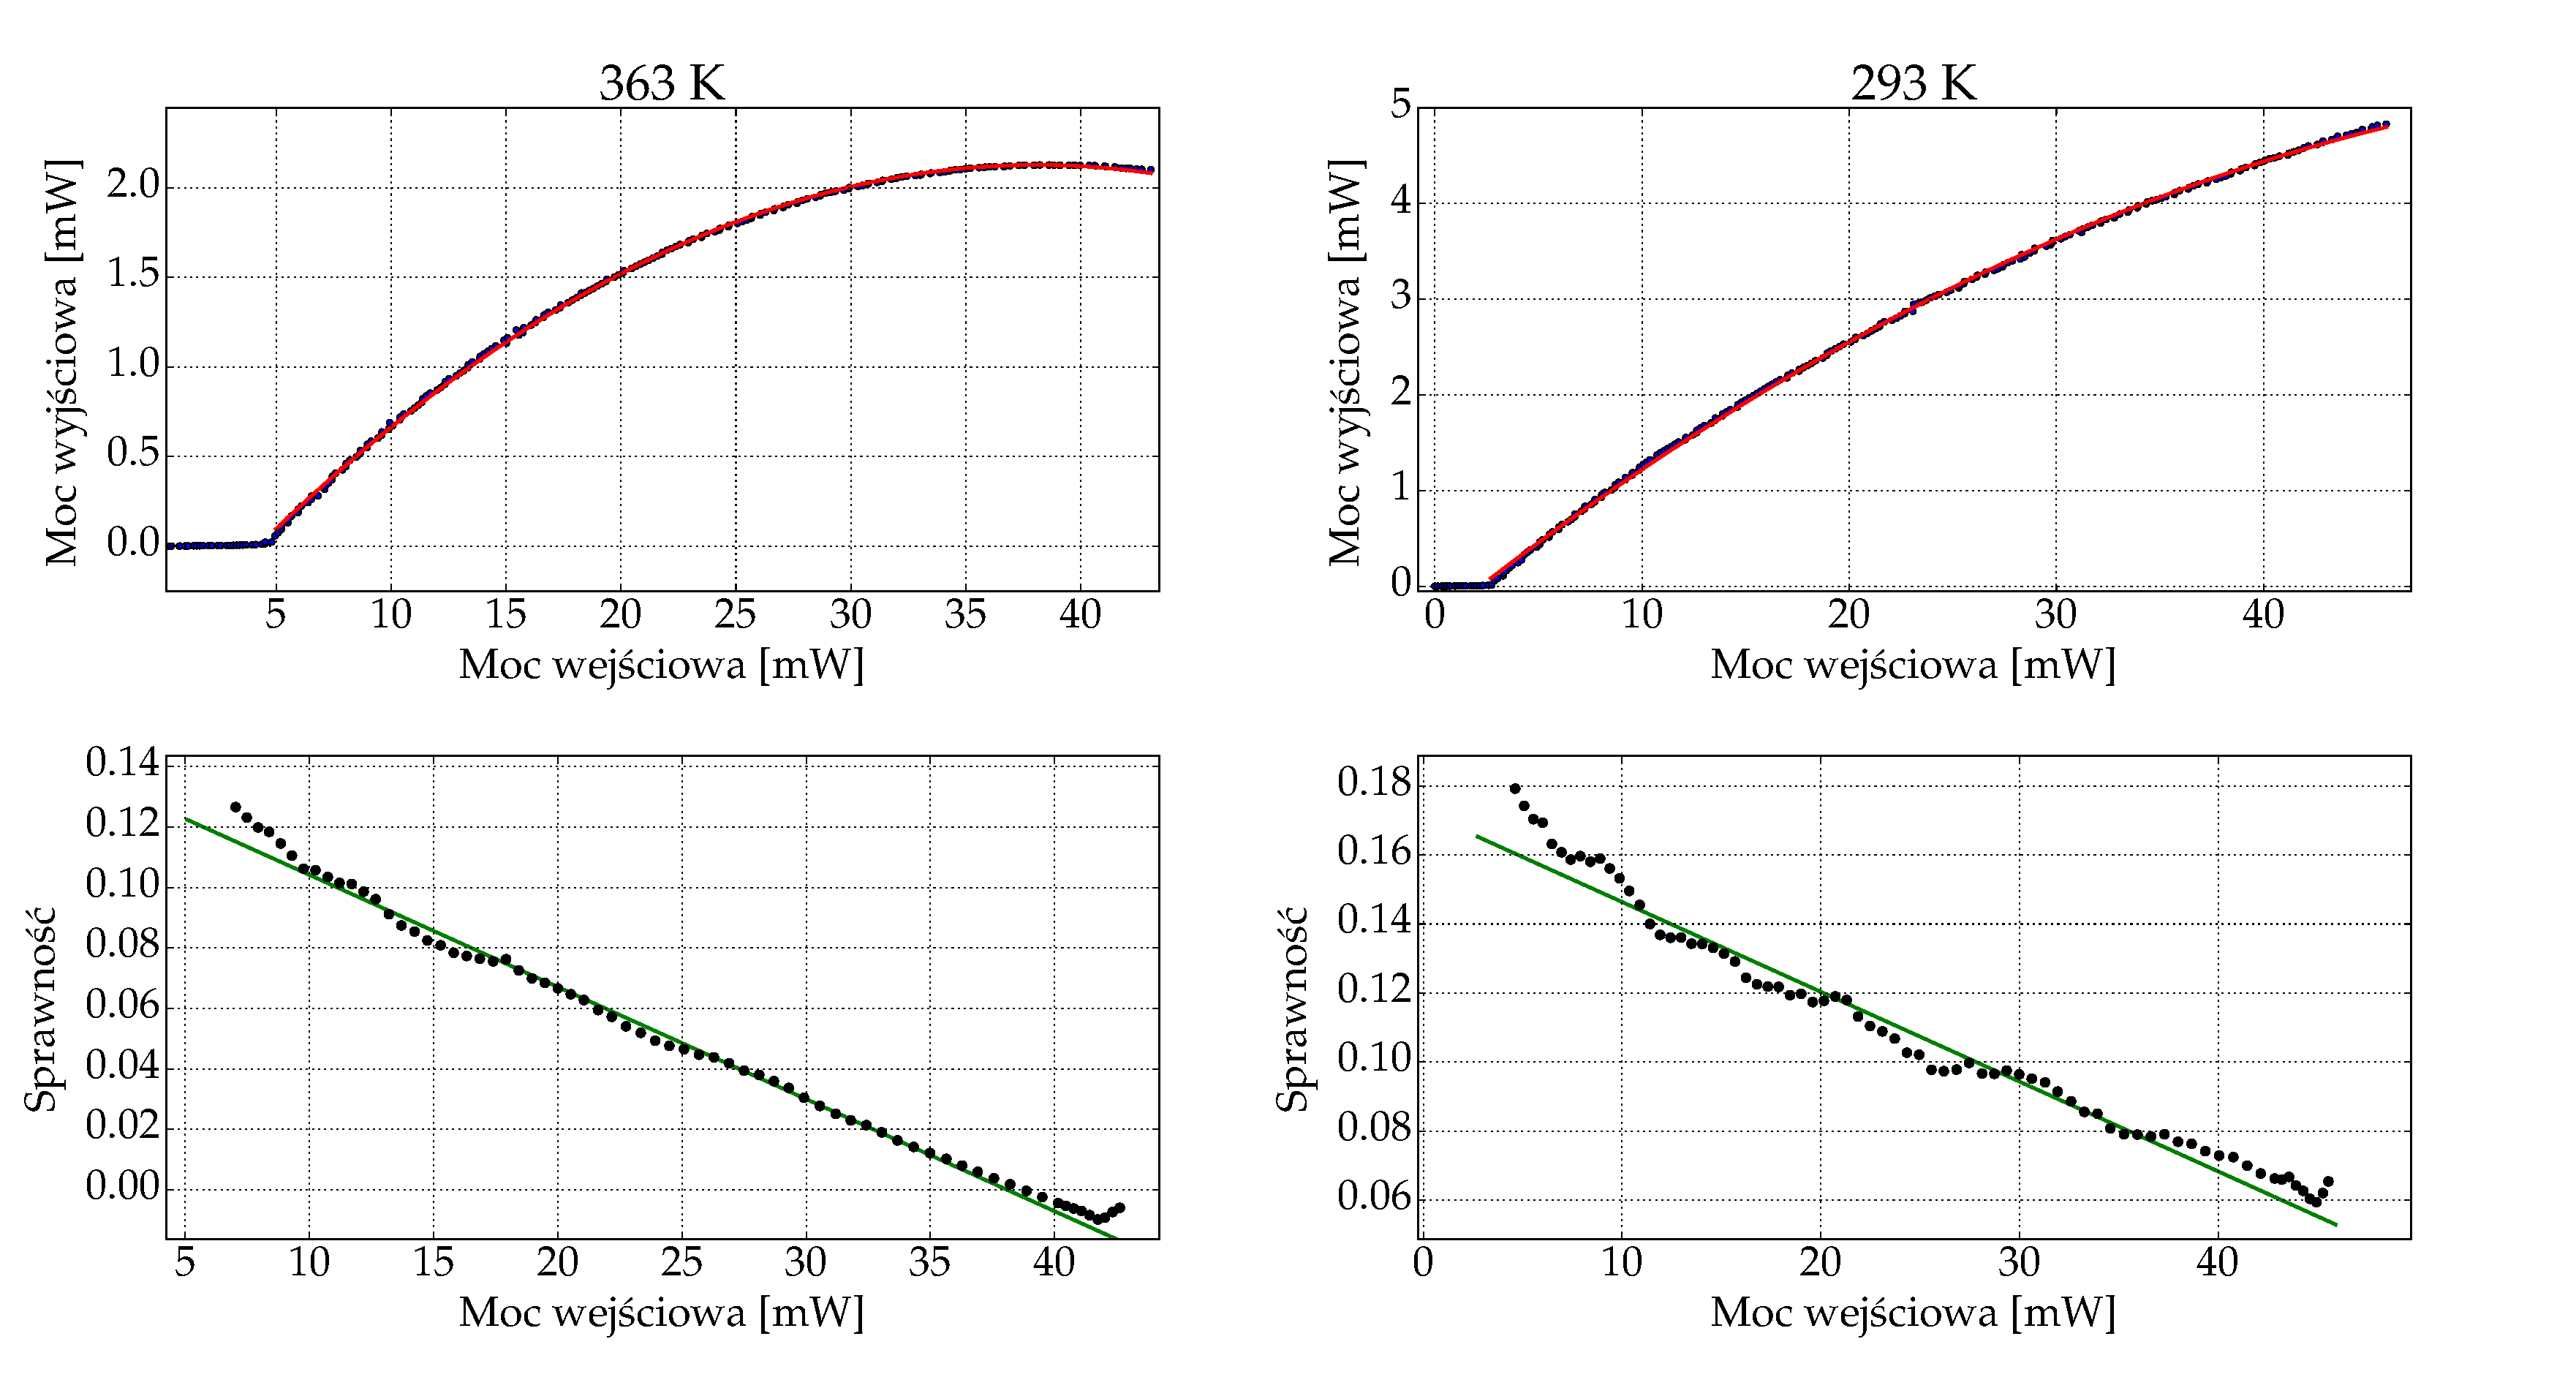
\includegraphics[scale=0.30]{plot_vcsel_850/plot_eff_20_90_via_power.eps}
  \label{fig:rys4}
  \caption{Sprawność VCSEL 850 dla temperatury 293\,K i 363\,K.} 
\end{figure}
\begin{figure}
\center
  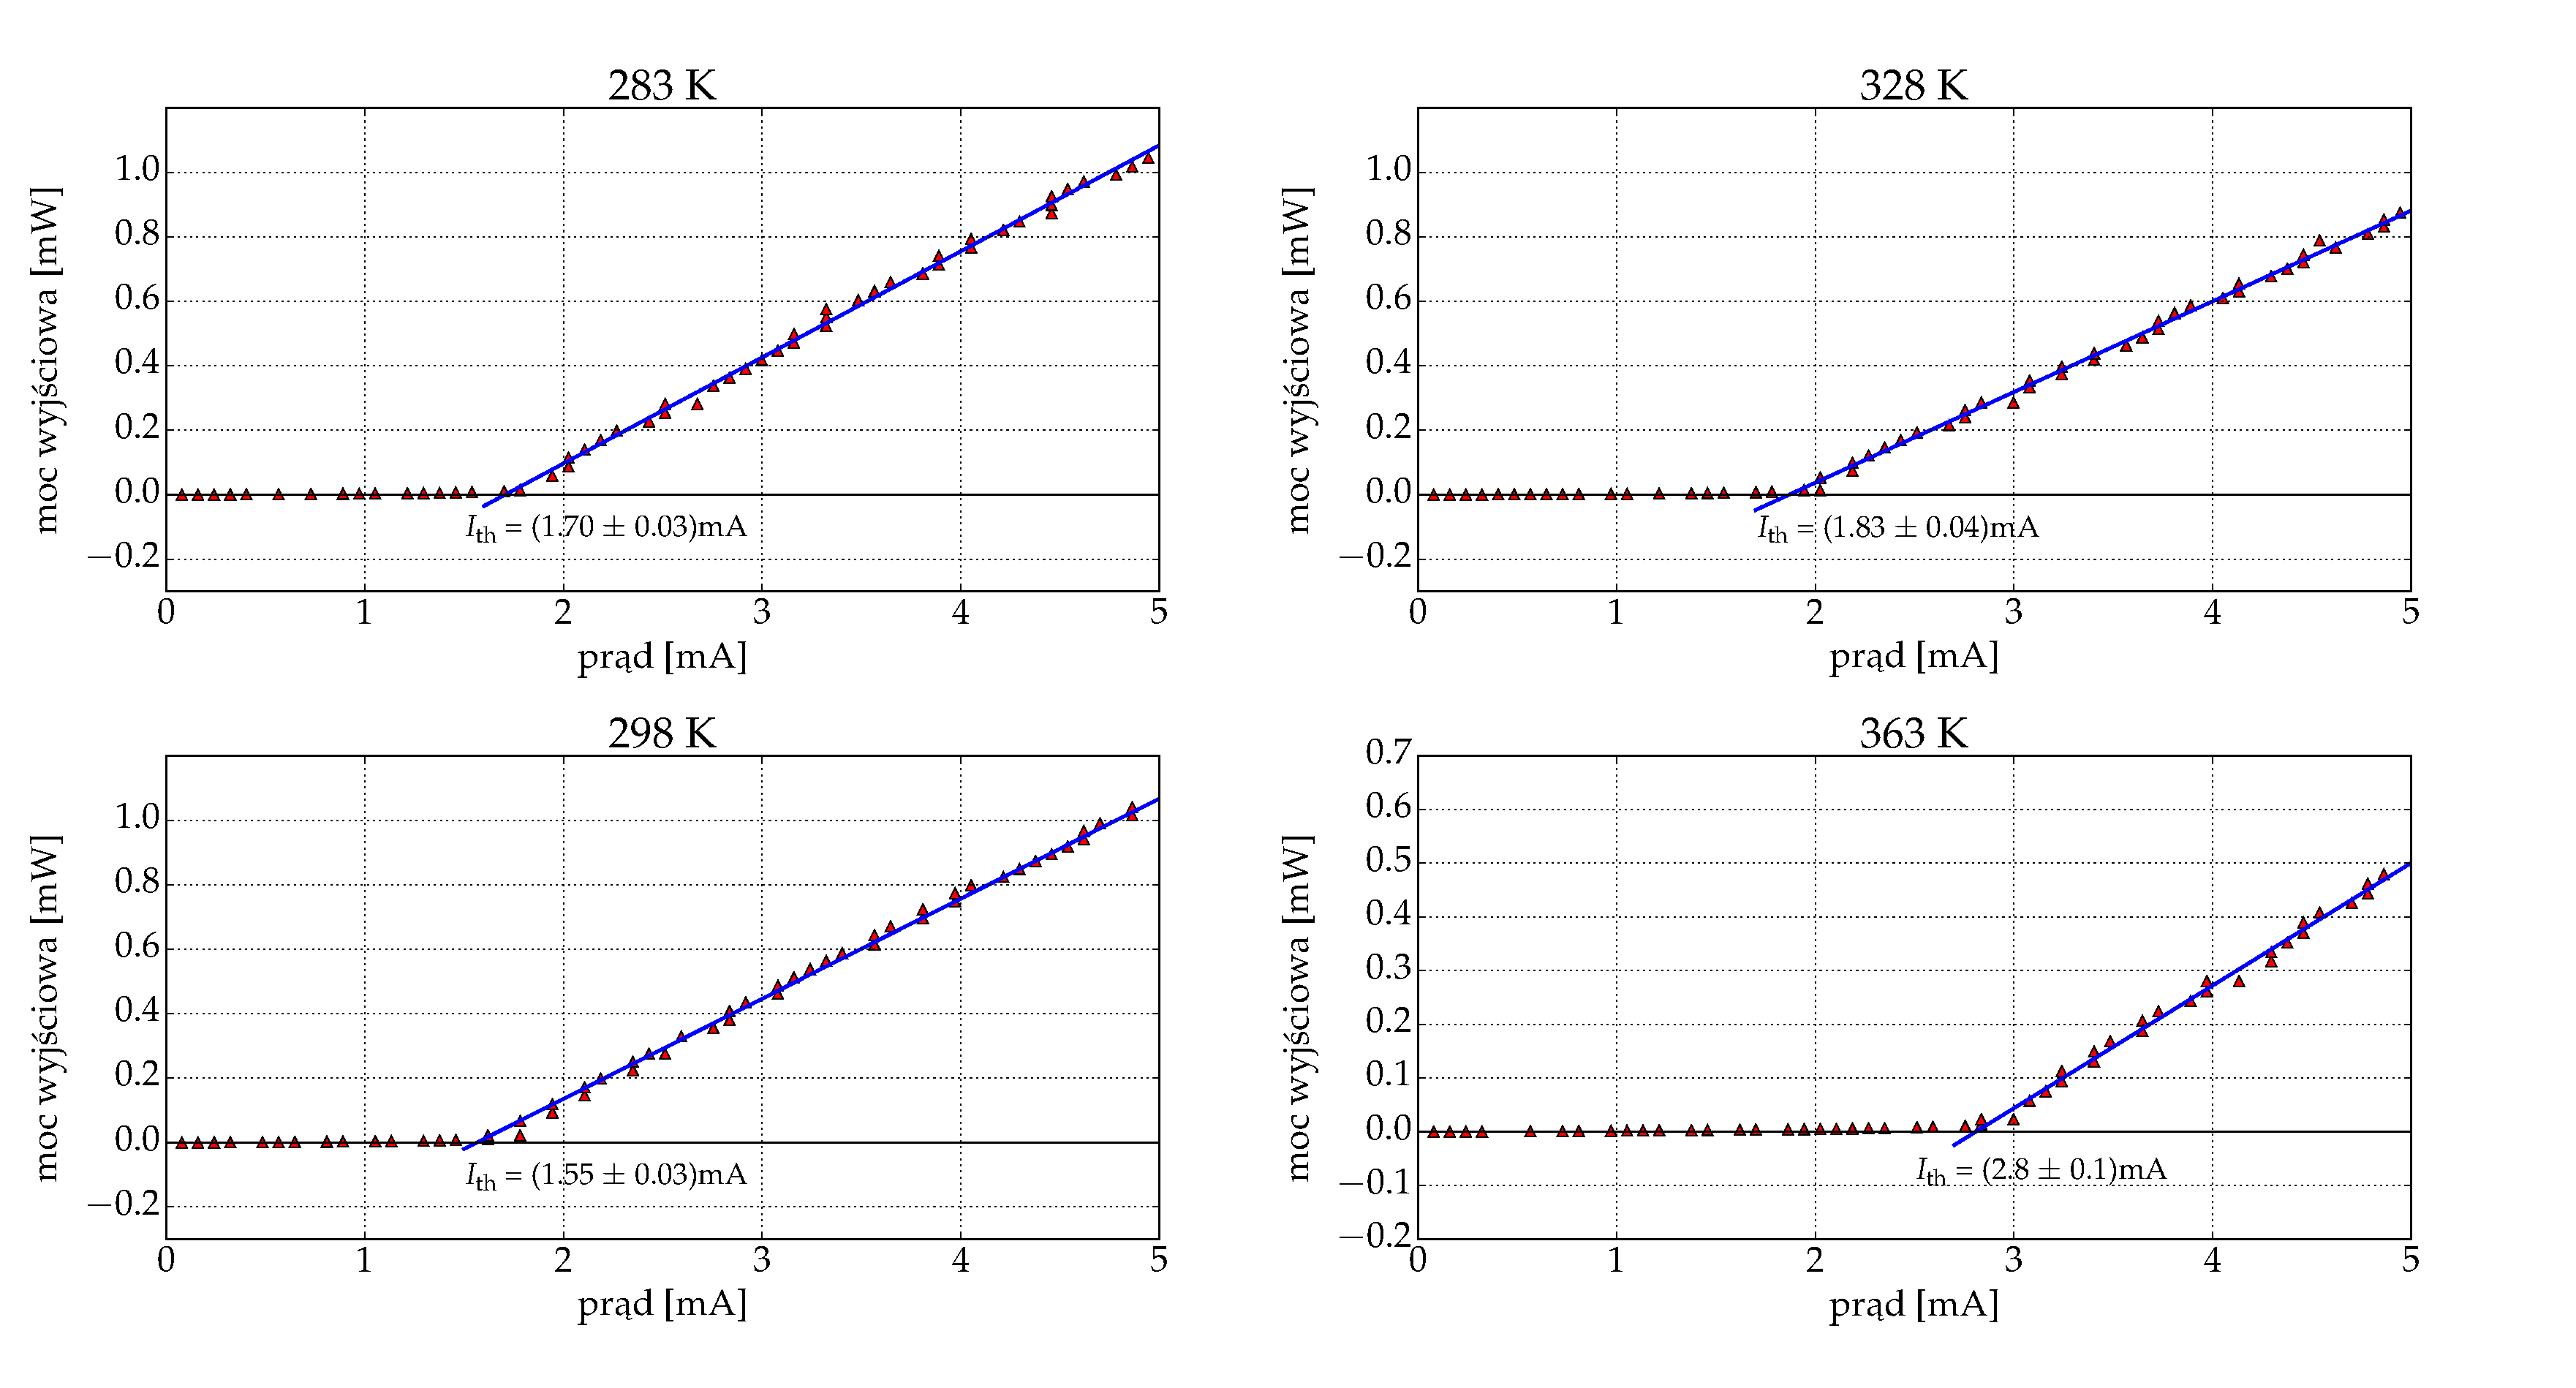
\includegraphics[scale=0.30]{plot_vcsel_850/plot_fit_i_th.eps}
  \caption{Wykres prądu progowego od temperatury z wyznaczonymi progami prądu.}
  \label{fig:rys5}
\end{figure}
\begin{figure}
\center
  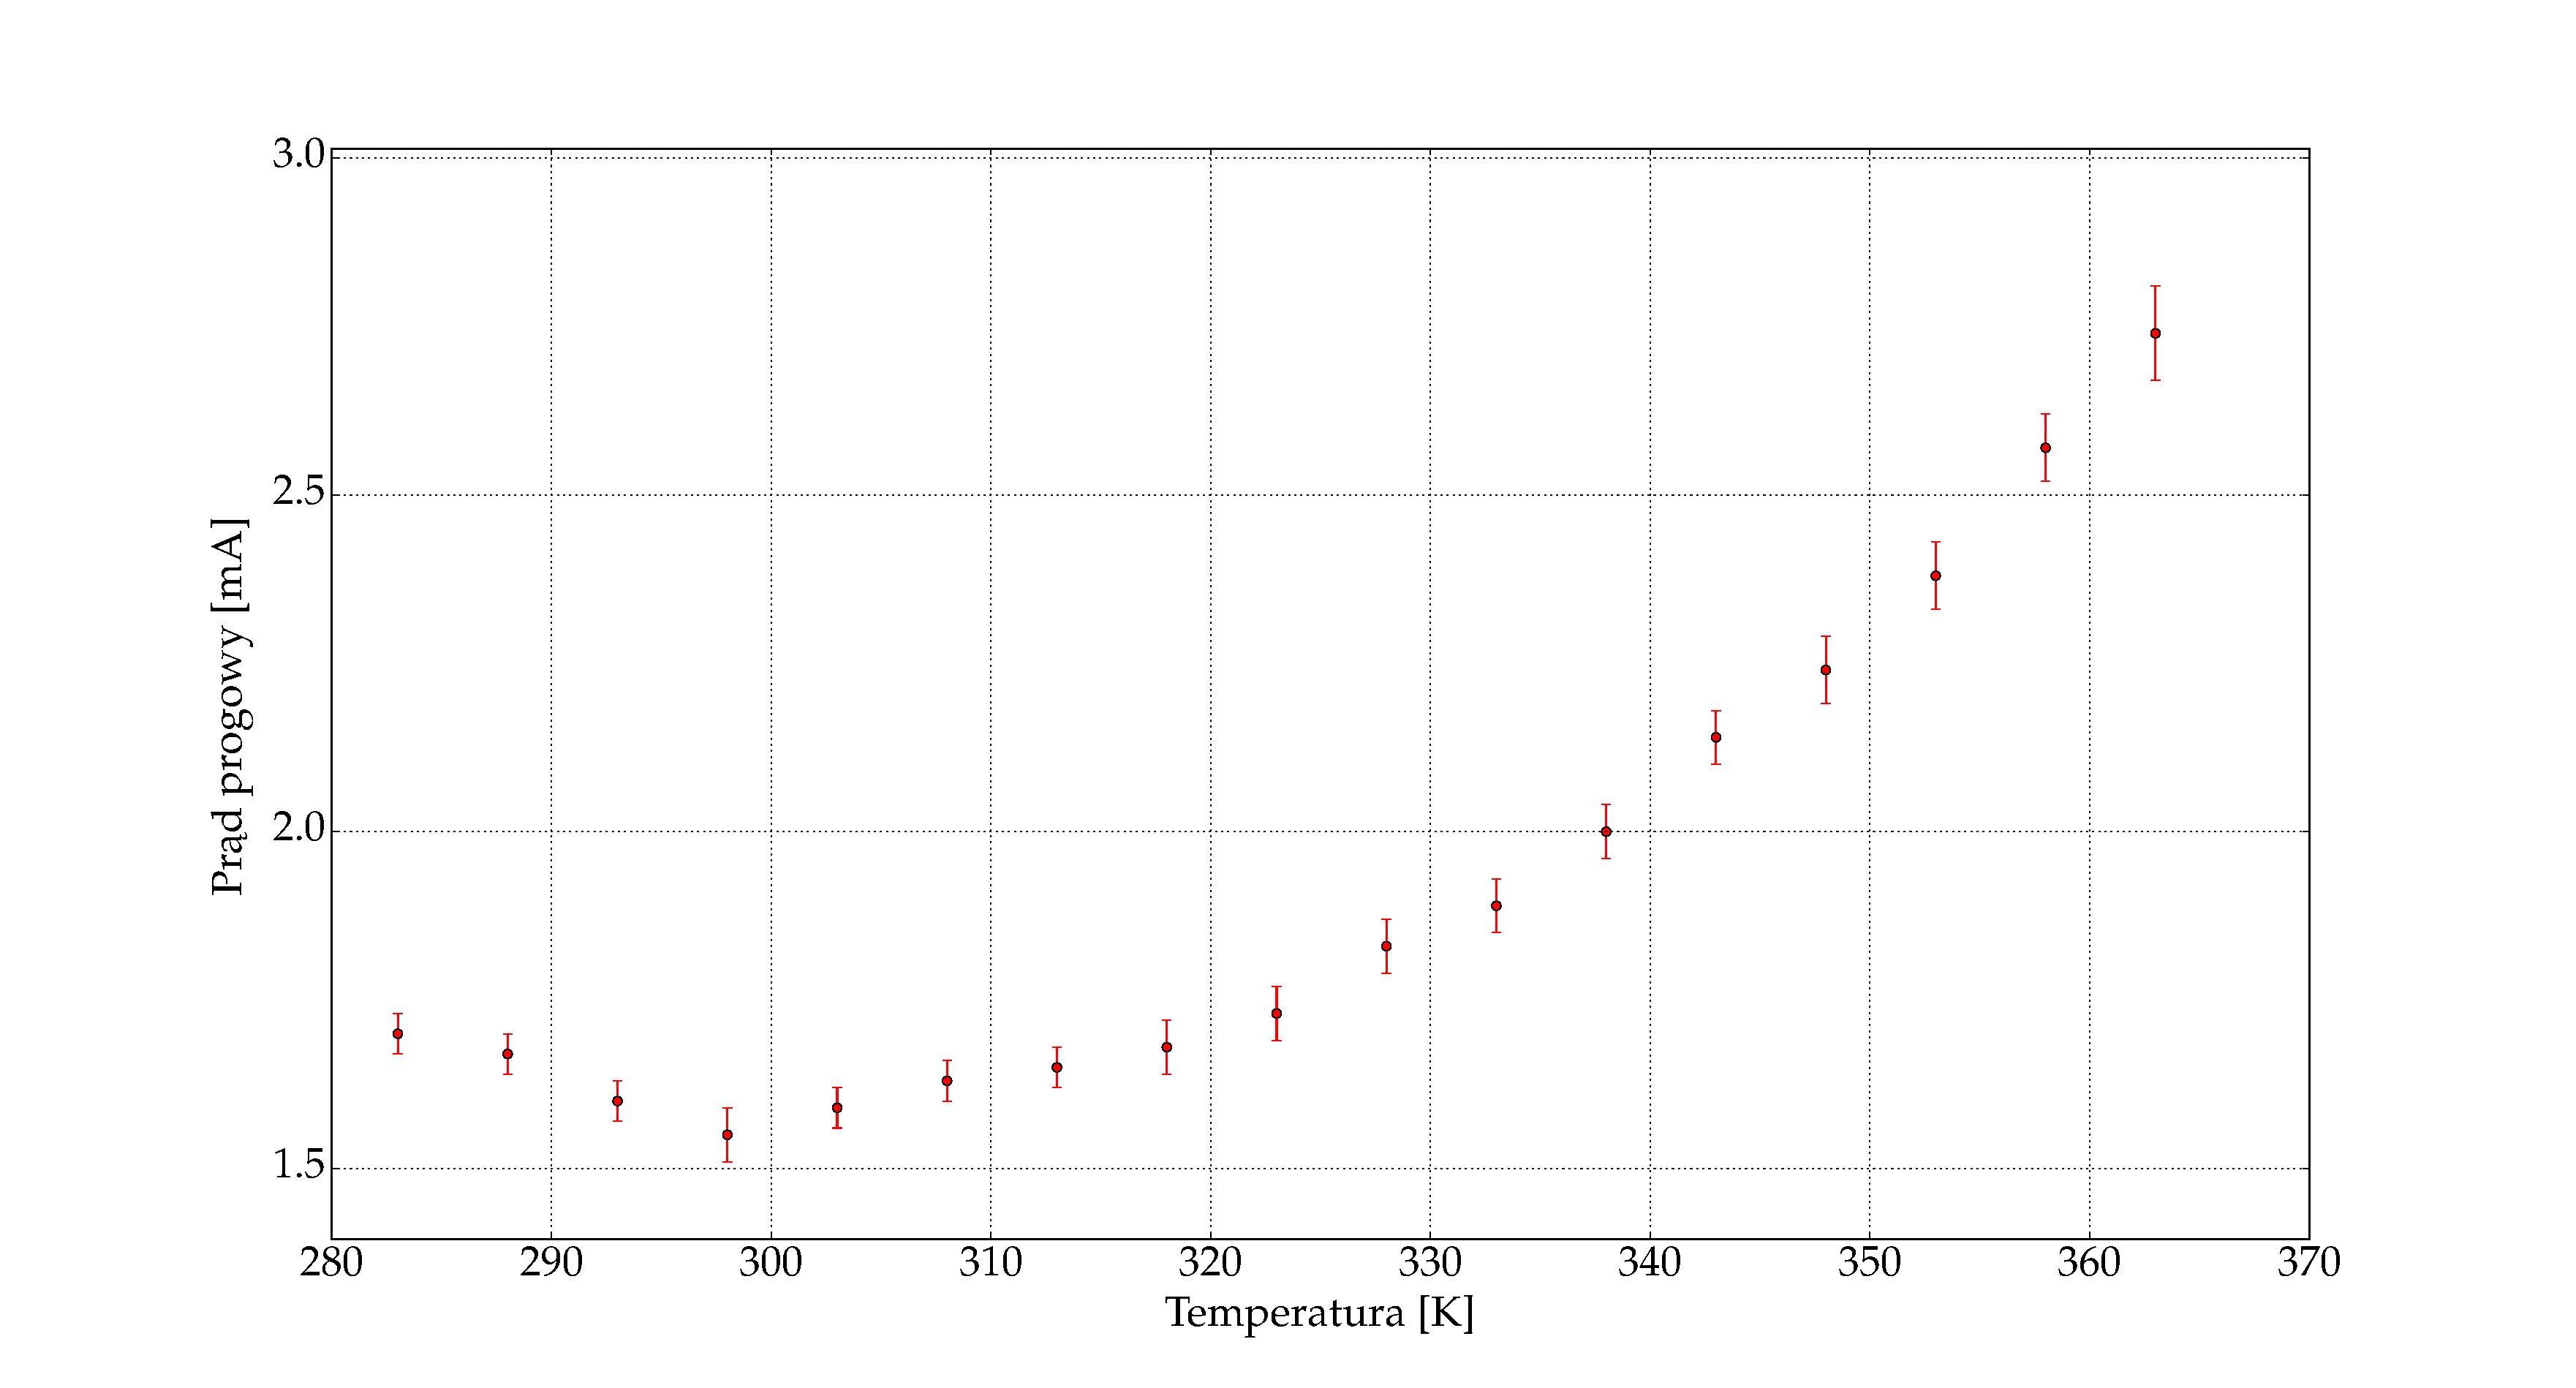
\includegraphics[scale=0.30]{plot_vcsel_850/plot_temp_i_th.eps}
  \caption{Wykres prądu progowego od temperatury.}
  \label{fig:rys6}
\end{figure}
